\documentclass[12pt,a4paper]{report}
\usepackage[utf8]{inputenc}
\usepackage{amsmath}
\usepackage{amsfonts}
\usepackage{amssymb}
\usepackage{graphicx}
\usepackage{lmodern}

\linespread{2}

\author{Kyle Swanson}
\title{Lab 4: Logic Breadboard}

\begin{document}
\maketitle

\paragraph{}
For this lab, we focused heavily on breadboards. We had a simple launchpad application that would "walk" several IO ports from the binary number 0000 to 1111. The first step was representing this on the breadboard. We used LEDs in a vertical configuration as shown in figure 1. Starting from the right we had bit 0, then 1, and so on. \\
\begin{figure}
	\centering
	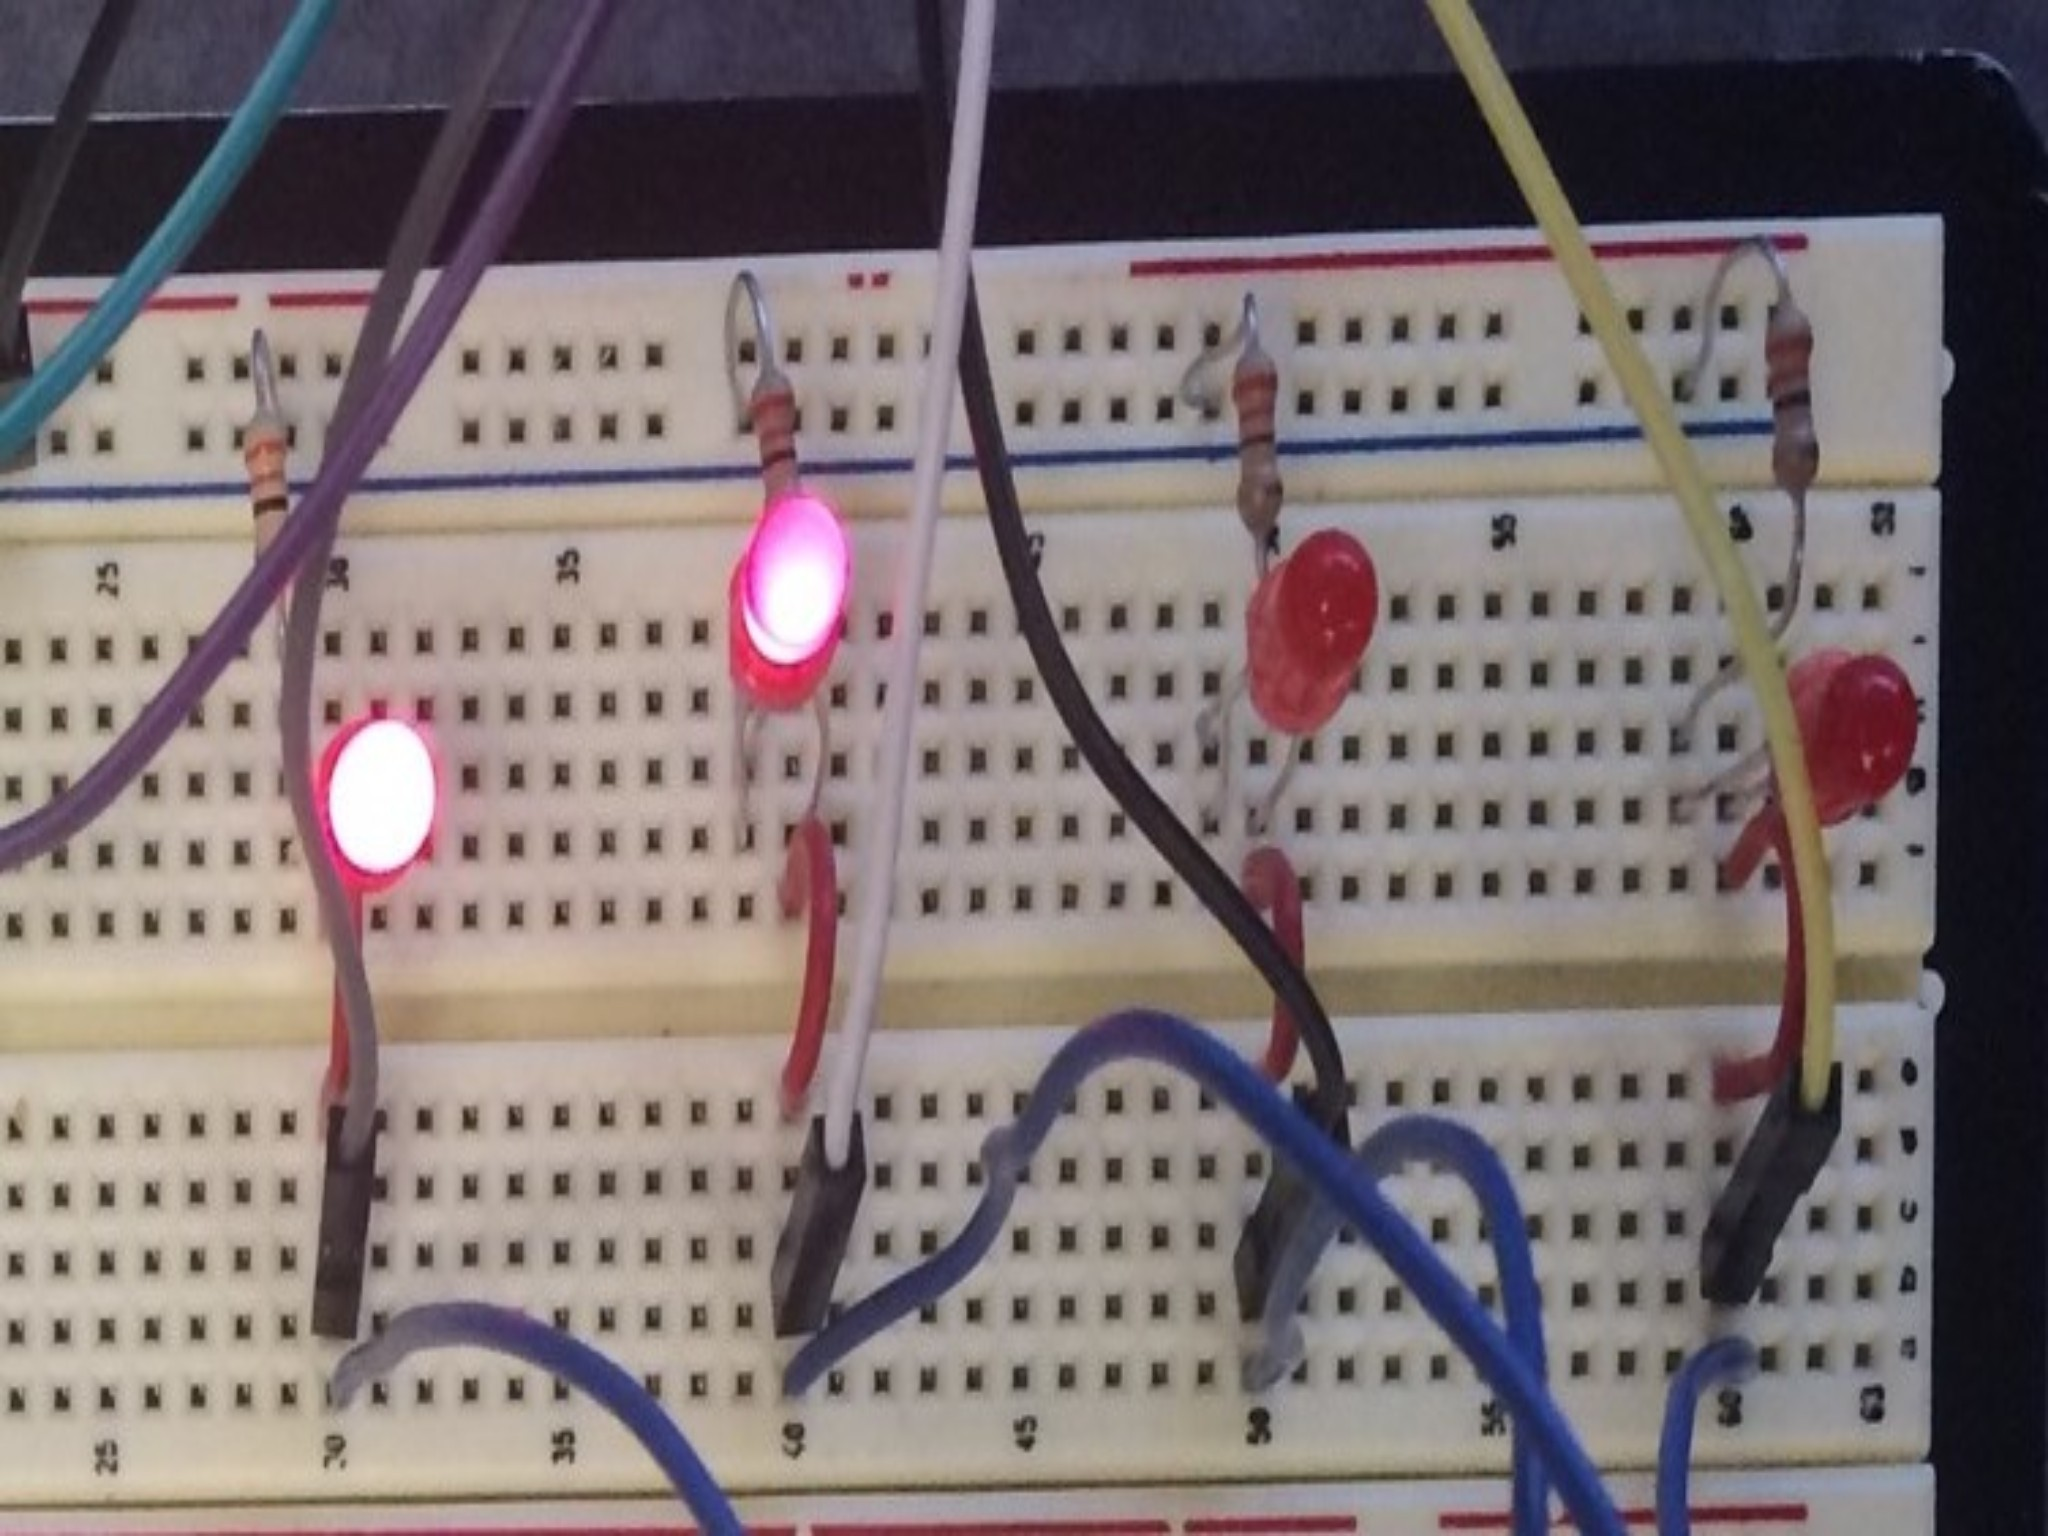
\includegraphics[scale=.1]{img/led_config} \\
	\caption{Our LED Arrangement}
\end{figure}

\paragraph{} 
The first step was building the circuits we needed for these experiments. We went through several iterations of our layout and colouring schemes when building. Quickly we learned how crucial the layout was in maintaining even a small breadboard. 
\paragraph{}
Eventually we completed the first step, so next we started implementing the 4-bit D Latch. We were using a 74LS75 D Latch. A D Latch is like a tiny bit of memory, you provide it input lines and output lines, and when you set an enable, it stores the value of the input lines. With our system we were storing 4 bits of information at a time. 

\begin{figure}
	\centering
	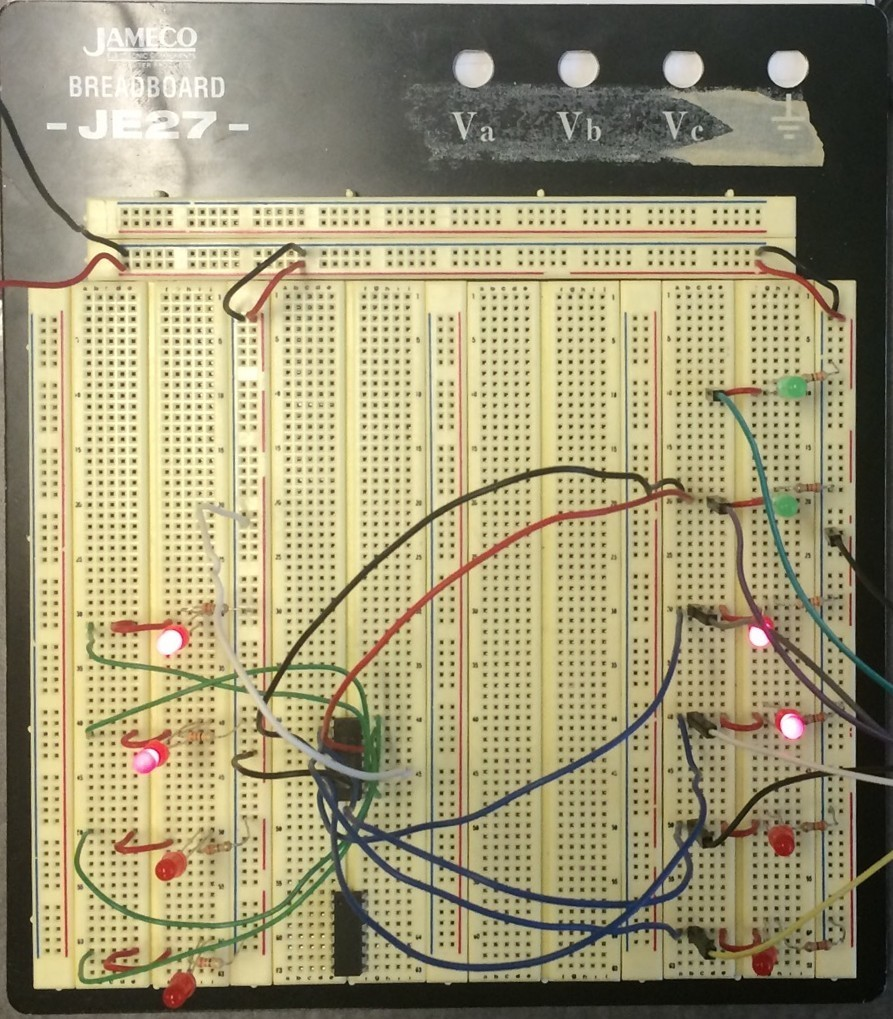
\includegraphics[scale=.3]{img/finished_latch} \\
	\caption{A Basic D Latch	}
\end{figure}

\paragraph{}
Like I said earlier, color coordination among our lines was critical. After our first iteration, we rewired it so that input lines were one color, and output were another color. This helped us keep track of what went where. Note Figure 2 for our final configuration.  

\paragraph{}
The D Latch was a good introduction to how this system could store small amounts of data. Using the Launchpad's controls, you could set the data bits on the right, then using an enable line, flash that to the D Latch. Then the bits on the left would stay at the D Latches values, even as you changed the right bits. 

\begin{figure}
	\centering
	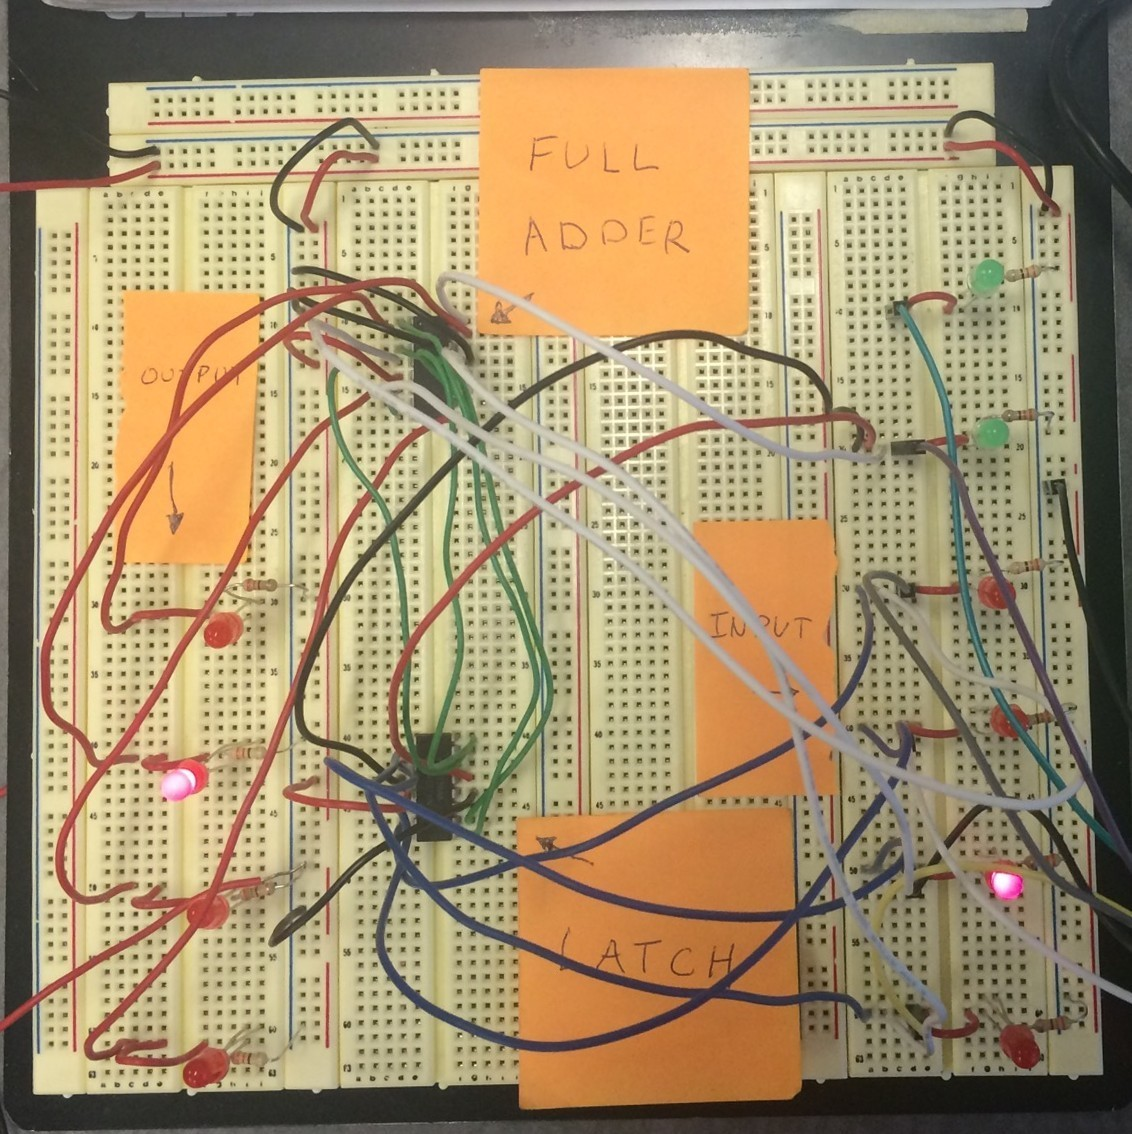
\includegraphics[scale=.3]{img/finished_adder} \\
	\caption{A Binary Adder	}
\end{figure}

\paragraph{}
Now that we had a working D Latch, we moved onto the adder. Adders, as the name implies, add binary bits. For our experiment, we wanted to add the stored value of the D Latch to the value of the bits the launchpad was controlling. For example if you stored 0011 in the D Latch, and set the right led bits to 0001, you would have the result 0100 on the left bits. See Figure 3 for our completed Adder. 

\paragraph{}
While working through the adder experiment we encountered a very strange, but predictable bug. If you set the D Latch to the binary value 0000, then counted on the right bus, the value wouldn't count properly. For example, it would could 0001, 0010, 0011, then return to 0000. However, the 2nd iteration after you counted through 4, it would count correctly. That is, to 1111 or 15. We tried replacing the Adder and D Latch to no avail. I think this illustrated how difficult building even simple circuits with a bread board can be. 

\paragraph{} 
For the final experiments, we used several more chips in place of the Adder to illustrate different boolean algebra theorems. We used a 74LS04 Hex Inverter, 74LS08 Quad 2-Input AND Gate, 74LS32 Quad 2-Input OR Gate, and finally implementing parts of DeMorgan's and the Covering Theorem. Like with the Adder these required us to wire the inputs and outputs correctly, and then you could see the results of the right bus and the latch reflected on the left bus. 

\paragraph{}
I found these experiments to be a helpful physical example of how bits work with boolean algebra. While I had done the math and even coded examples before, it was exciting to see the actual output on led. It really made me appreciate the complexity of using different chips for different types of gates. The complexity of even the most simple AND gate is astounding. 


\end{document}